\documentclass[10pt]{amsart}
\usepackage{amsmath}
\usepackage{amssymb}
\usepackage{tikz}
\usetikzlibrary{arrows}

\begin{document}

\begin{center}
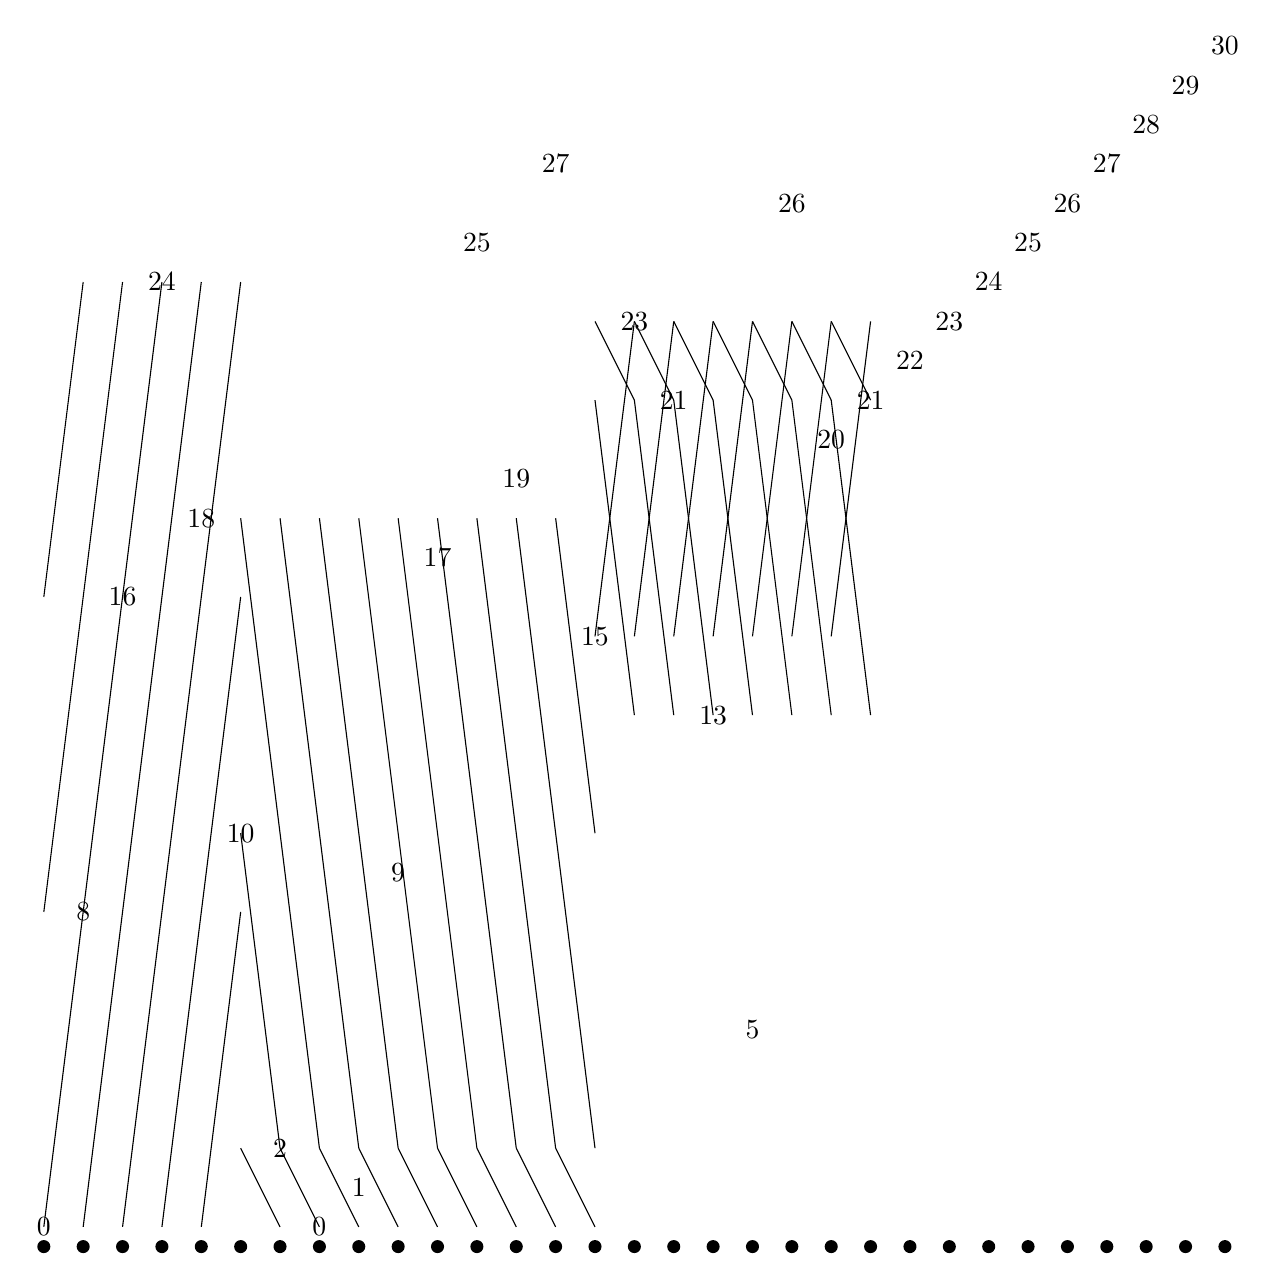
\begin{tikzpicture}[scale=.5]
% Nodes
\foreach \x/\y in {0/0,1/8,2/16,3/24,4/18,5/10,6/2,7/0,8/1,9/9,10/17,11/25,12/19,13/27,14/15,15/23,16/21,17/13,18/5,19/26,20/20,21/21,22/22,23/23,24/24,25/25,26/26,27/27,28/28,29/29,30/30}{%
\draw (\x,-.5) node[circle, fill=black, scale=0.5] {};
\node at (\x,\y){$\y$};
}
% Lines
\foreach \x in {0,...,4}{
\draw (\x,0)--(\x+1,8);
\draw (\x,8)--(\x+1,16);
\draw (\x,16)--(\x+1,24);
}
\foreach \x in {5,...,13}{
\draw (\x,18)--(\x+1,10);
\draw (\x,10)--(\x+1,2);
\draw (\x,2)--(\x+1,0);
}
\foreach \x in {14,...,20}{
\draw (\x,15)--(\x+1,23);
\draw (\x,23)--(\x+1,21);
\draw (\x,21)--(\x+1,13);
}
\end{tikzpicture}
\captionof{figure}{Linear realizations for $\{1^6,7^{18}\}$ and $\{1^7,7^{17},8^3\}$.}
\end{center}

\end{document}